\section{Chapter 4: Labor Market Equilibrium}

This chapter will study the notion of labor market equilibrium,
which is the outcome of the interaction between labor supply, labor demand,
and possibly external forces, such as government policies.


\begin{definition}[Invisible Hand Theorem] 
    
    If markets are competitive, and workers and 
    firms are free to enter and leave the market, then 
    the equilibrium allocation of workers and wages 
    will be efficient, in the sense that it maximizes 
    the total gains that workers and firms 
    obtain from trade with each other.

\end{definition}

%%%%%%%%%%%%%%%%%%%%%%%%%%%%%%%%%%%%%%%%%%%%%%%%%%%%%%%%%%%%%%%%%%%%%%%%%%%%%%%%%%%%%%%
%%%%%%%%%%%%%%%%%%%%%%%%%%%%%%%%%%%%%%%%%%%%%%%%%%%%%%%%%%%%%%%%%%%%%%%%%%%%%%%%%%%%%%%
\subsection{Equilibrium in a Single Labor Market}

\autoref{fig:ch_4p1_surplus}
illustrates a competitive labor market with an 
equilibrium at $(E^*, w^*)$.


\FloatBarrier

\begin{figure}[!htb]
    \centering
        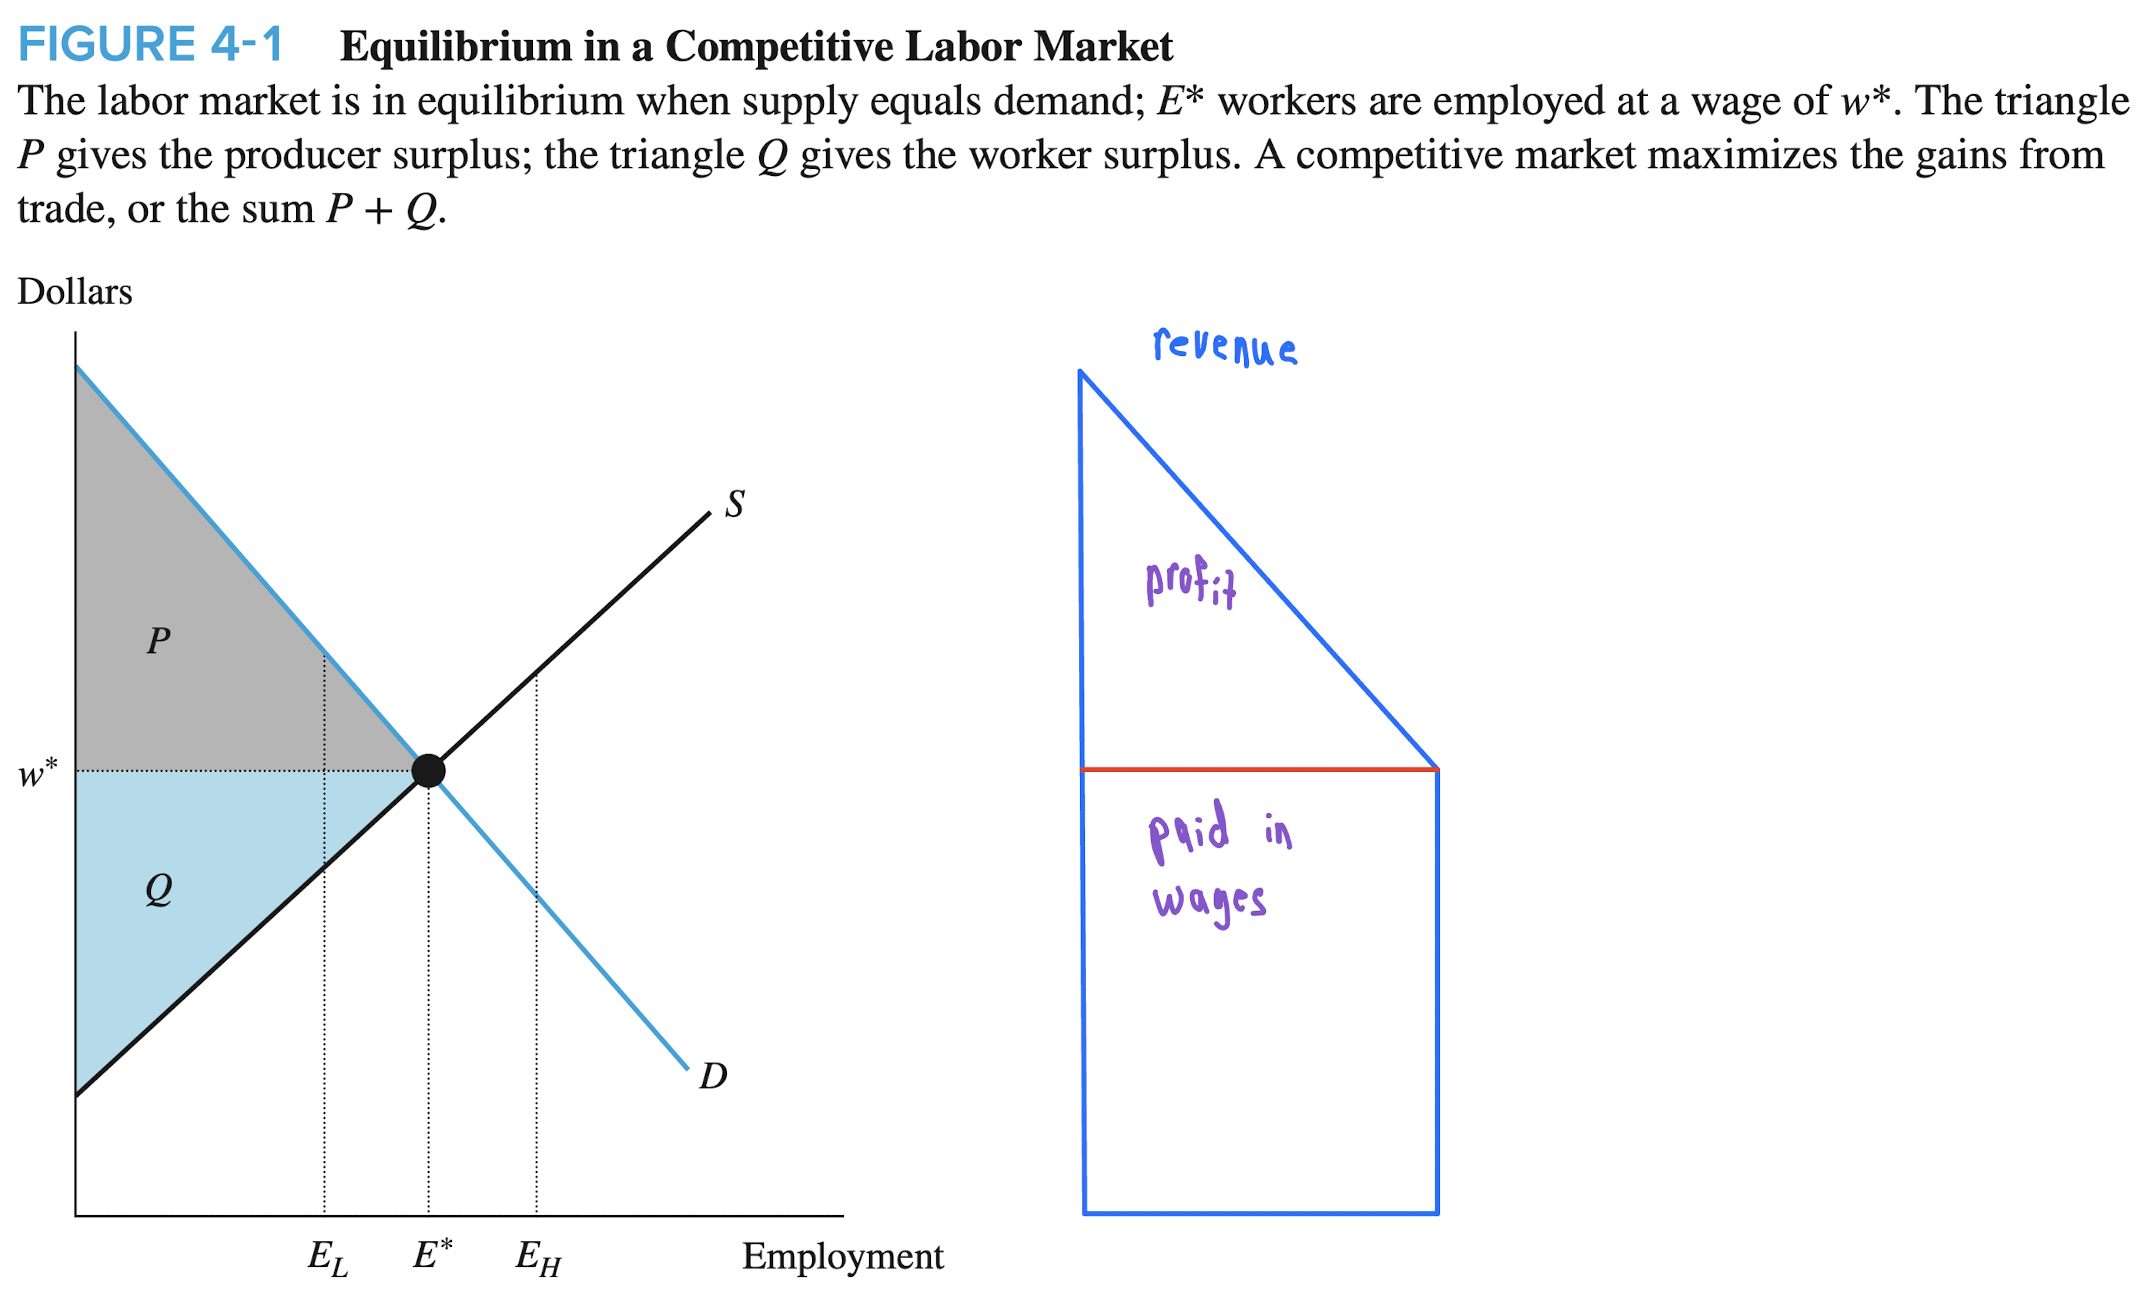
\includegraphics[width=0.95\textwidth]{../input/ch_4p1_surplus.png}
    \caption{Labor Market Surplus}
    \label{fig:ch_4p1_surplus}
\end{figure}

\FloatBarrier

Since the labor demand curve corresponds to the value of 
the marginal product, we can see that the area under the labor 
demand curve up to any given point corresponds to the total revenue
a firm receives from hiring that many workers.
Thus, since the equilibrium is at $(E^*, w^*)$, the
firm's total revenue is given by the area under the demand 
curve up to $E^*$, which is drawn out 
in blue in \autoref{fig:ch_4p1_surplus}.
Similarly, the area under the supply curve up to $E^*$,
their profit, or producer surplus (denoted $P$ in \autoref{fig:ch_4p1_surplus}), is 
given by the triangle above $w^*$ and below the labor 
demand curve.

\begin{definition}[Producer Surplus] 

    Producer surplus is the difference between the 
    revenue a firm receives and the cost it incurs.
    
\end{definition}

Similarly, workers are indifferent between working and not working 
along the labor supply curve. Thus, workers who are 
willing to work for less than $w^*$ (which is everyone 
except the final workers hired) receive a surplus.
This surplus is given by the triangle below $w^*$ and
above the labor supply curve, denoted $Q$ in 
\autoref{fig:ch_4p1_surplus}.

The gains from trade are given by the sum of the
producer and worker surplus: $P + Q$.
The competitive market equilibrium maximizes the 
gains from trade. Such an outcome that maximizes 
gains from trade is said to be ``efficient.''

\begin{questions}
    It's somewhat challenging for me to think about 
    how I should think about the connection between surplus 
    and wellbeing. I understood surplus as a clear quantitative 
    measure, but it seems like we would only care about it insofar as it 
    connects to something more like the wellbeing of the parties 
    involved. However, it's super unclear to me 
    if we're trying to connect it back to that 
    in any way.
\end{questions}

%%%%%%%%%%%%%%%%%%%%%%%%%%%%%%%%%%%%%%%%%%%%%%%%%%%%%%%%%%%%%%%%%%%%%%%%%%%%%%%%%%%%%%%
%%%%%%%%%%%%%%%%%%%%%%%%%%%%%%%%%%%%%%%%%%%%%%%%%%%%%%%%%%%%%%%%%%%%%%%%%%%%%%%%%%%%%%%
\subsection{Equilibrium across Labor Markets}

So far, we have focused on a single labor market.
Now, we turn to the case of multiple labor markets
linked by migration.
In \autoref{fig:ch_4p2_multiple_markets},
we see two labor markets, $N$ (north) and $S$ (south).
We start with the wages ($w_n$) in the north being 
higher than the wages ($w_s$) in the south.
If workers are able to move freely, then workers 
from the South will move to the North, which will
decrease supply in the South and increase supply
in the North up to the point that wages are equalized
across the two markets, at $w^*$.
Note that this analysis relies on the idea that workers 
in each region are perfect substitutes for each other.

We find that this movement 
increases the total output across the markets.
Specifically, the North market's 
output is originally the area under the demand curve 
up to $A$ and after the move extends to $B$ -- the 
increase is characterized by the blue trapezoid.
For the South, output reduces by the amount characterized 
by the blue trapezoid in its market. However,
the increase in the North is larger than the decrease
in the South. In particular, the growth in the North
is large by the size of the triangle $ABC$.


\FloatBarrier

\begin{figure}[!htb]
    \centering
        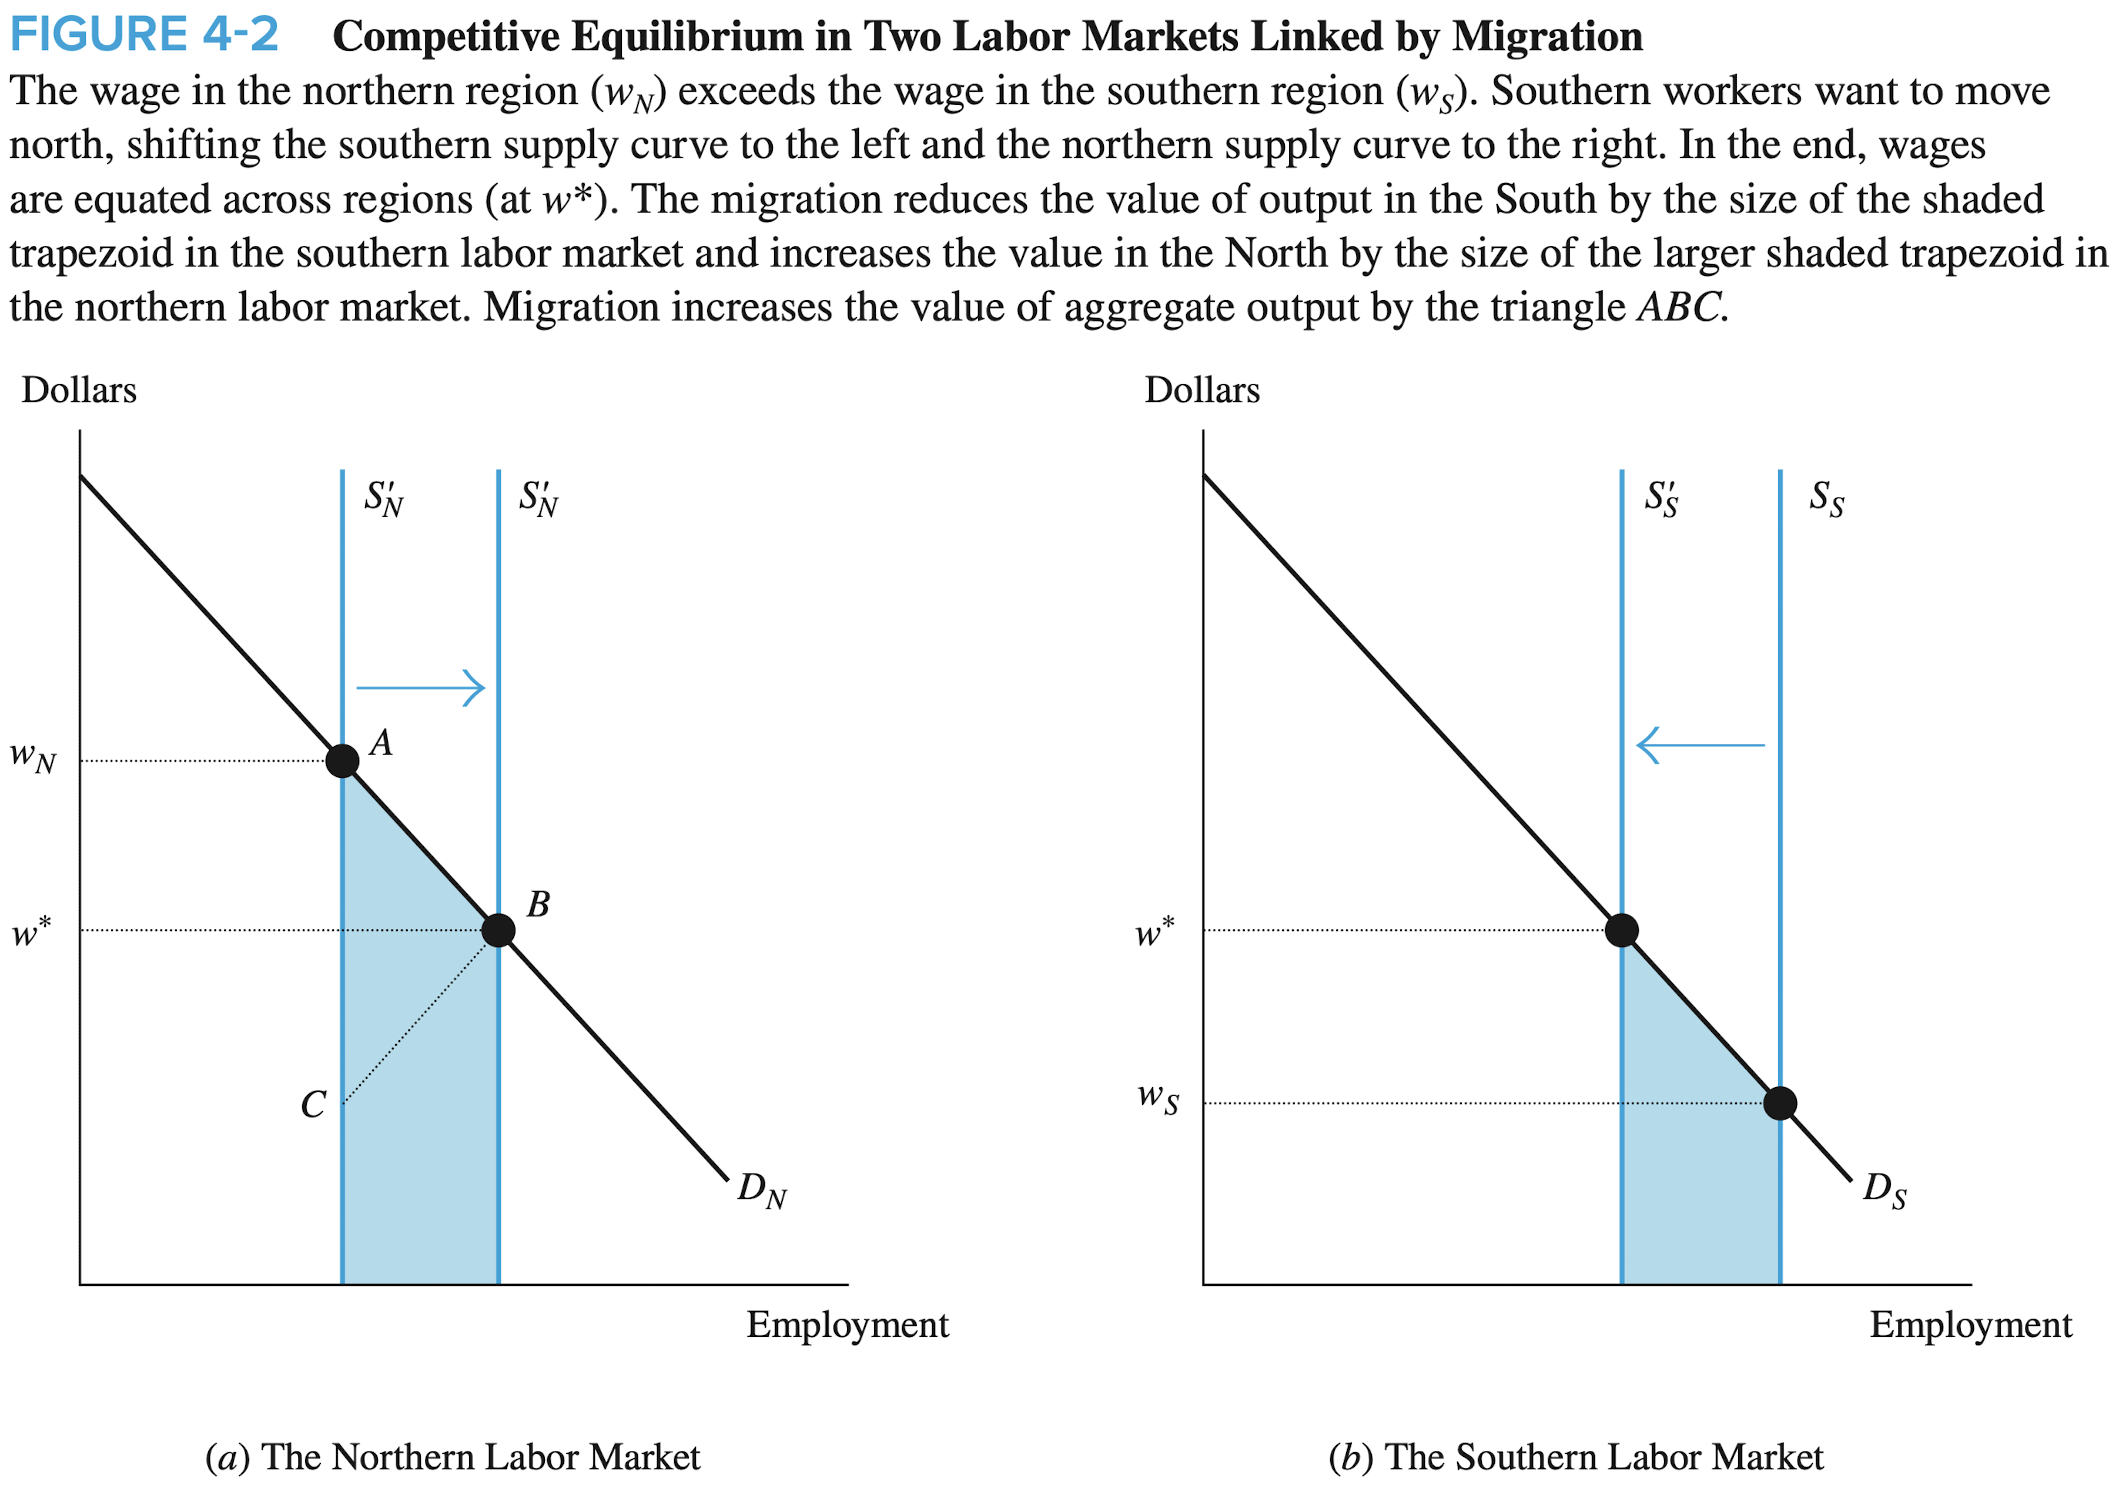
\includegraphics[width=0.95\textwidth]{../input/ch_4p2_multiple_markets.png}
    \caption{Equilibrium across Labor Markets}
    \label{fig:ch_4p2_multiple_markets}
\end{figure}

\FloatBarrier


%%%%%%%%%%%%%%%%%%%%%%%%%%%%%%%%%%%%%%%%%%%%%%%%%%%%%%%%%%%%%%%%%%%%%%%%%%%%%%%%%%%%%%%
%%%%%%%%%%%%%%%%%%%%%%%%%%%%%%%%%%%%%%%%%%%%%%%%%%%%%%%%%%%%%%%%%%%%%%%%%%%%%%%%%%%%%%%
\subsection{Policy Application: Payroll Taxes and Subsidies}

\subsubsection{Payroll Taxes Imposed on the Firm}

The payroll tax is a tax imposed on the firm 
that is some fraction $\tau$ of the wage paid to
the worker.

\autoref{fig:ch_4p3_payroll_tax}
illustrates the effect of a payroll tax.
Here, we suppose there is a payroll tax of \$1 per hour.
The initial equilibrium is at $(E_0, w_0)$, at point $A$.
The payroll tax placed on the firm decreases
the labor demand uniformly by the amount of the tax.
Thus, the new equilibrium is at point $B$, where 
the employment level is now $E_1$, the wage received 
by the worker is $w_1$, and the effective wage paid by 
the firm is $w_1 + 1$.

\FloatBarrier

\begin{figure}[!htb]
    \centering
        \includegraphics[width=0.95\textwidth]{../input/ch_4p3_payroll_tax.png}
    \caption{Payroll Tax}
    \label{fig:ch_4p3_payroll_tax}
\end{figure}

\FloatBarrier

%%%%%%%%%%%%%%%%%%%%%%%%%%%%%%%%%%%%%%%%%%%%%%%%%%%%%%%%%%%%%%%%%%%%%%%%%%%%%%%%%%%%%%%
\subsubsection{Payroll Taxes Imposed on the Worker}

\autoref{fig:ch_4p3_payroll_tax_worker}
illustrates the effect of a payroll tax
if it were imposed on the worker instead of the firm.
Here, the effect is essentially the reverse
in which the labor supply curve shifts up 
by the amount of the tax.
Now, the equilibrium is 
at point $B$, where the employment level is $E_1$,
the wage received by the worker is $w_1$, but 
the worker now pays a tax such that the 
effective wage received by the worker becomes $w_1 - 1$.

Whether the tax is imposed on the firm or the worker,
the outcome is the same.

\FloatBarrier

\begin{figure}[!htb]
    \centering
        \includegraphics[width=0.95\textwidth]{../input/ch_4p3_payroll_tax_worker.png}
    \caption{Payroll Tax Imposed on Workers}
    \label{fig:ch_4p3_payroll_tax_worker}
\end{figure}

\FloatBarrier

%%%%%%%%%%%%%%%%%%%%%%%%%%%%%%%%%%%%%%%%%%%%%%%%%%%%%%%%%%%%%%%%%%%%%%%%%%%%%%%%%%%%%%%

\subsubsection{When Will the Payroll Tax Be Shifted Completely to Workers?}

When the labor supply is perfectly inelastic,
the entire burden of the payroll tax is shifted to the worker,
as illustrated in \autoref{fig:ch_4p3_inelastic_and_payroll}.

\FloatBarrier

\begin{figure}[!htb]
    \centering
        \includegraphics[width=0.95\textwidth]{../input/ch_4p3_inelastic_and_payroll.png}
    \caption{When Payroll Tax is Shifted Completely to Workers}
    \label{fig:ch_4p3_inelastic_and_payroll}
\end{figure}

\FloatBarrier

%%%%%%%%%%%%%%%%%%%%%%%%%%%%%%%%%%%%%%%%%%%%%%%%%%%%%%%%%%%%%%%%%%%%%%%%%%%%%%%%%%%%%%%

\subsubsection{Deadweight Loss}

\autoref{fig:ch_4p3_deadweight_loss}
displays the reduction in the total surplus -- aka the deadweight loss --
that results from the imposition of a payroll tax.
Recall that the initial equilibrium is at $(E_0, w_0)$,
and the new equilibrium after the tax is at $(E_1, w_{\text{NET}})$,
where the firm pays $w_{\text{TOTAL}}$ and the worker receives $w_{\text{NET}}$.
Now, the total surplus has been reduced by the $DL$ triangle.
The consumer surplus now becomes
$Q^*$, rather than $Q$; the producer surplus now 
becomes $P^*$, rather than $P$; and the government
collects tax revenue equal to the rectangle $T$.

If you look back at \autoref{fig:ch_4p3_inelastic_and_payroll},
you can see that when the labor supply is perfectly inelastic,
there is no deadweight loss from the imposition of the tax,
and the producer surplus remains the same. 
All that changes is a transfer of consumer surplus to 
the government in the form of tax revenue. Specifically,
the rectangle characterized by $w_0AB(w_0 - 1)$
is transferred from consumer surplus to government revenue.


\FloatBarrier

\begin{figure}[!htb]
    \centering
        \includegraphics[width=0.95\textwidth]{../input/ch_4p3_deadweight_loss.png}
    \caption{Deadweight Loss}
    \label{fig:ch_4p3_deadweight_loss}
\end{figure}

\FloatBarrier